\documentclass[a4paper,uplatex,dvipdfmx]{jsarticle}

% ---Display \subsubsection at the Index
% \setcounter{tocdepth}{3}

% ---Setting about the geometry of the document----
% \usepackage{a4wide}
% \pagestyle{empty}

% ---Physics and Math Packages---
\usepackage{amssymb,amsfonts,amsthm,mathtools}
\usepackage{physics,braket,bm}

% ---underline---
\usepackage{ulem}

% ---cancel---
\usepackage{cancel}

% --- surround the texts or equations
% \usepackage{fancybox,ascmac}

% ---settings of theorem environment---
\usepackage{amsthm}
\theoremstyle{definition}
\newtheorem{dfn}{定義}
\newtheorem{prop}{命題}
\newtheorem{thm}{定理}

% ---settings of proof environment---
\renewcommand{\proofname}{\textbf{証明}}
\renewcommand{\qedsymbol}{$\blacksquare$}

% ---Ignore the Warnings---
\usepackage{silence}
\WarningFilter{latexfont}{Some font shapes,Font shape}
\ExplSyntaxOn
\msg_redirect_name:nnn{hooks}{generic-deprecated}{none}
\ExplSyntaxOff

% ---Insert the figure (If insert the `draft' at the option, the process becomes faster.)---
\usepackage{graphicx}
% \usepackage{subcaption}

% ----Add a link to a text---
\usepackage{url,hyperref}
\usepackage[dvipsnames,svgnames]{xcolor}
\hypersetup{colorlinks=true,citecolor=FireBrick,linkcolor=Navy,urlcolor=purple}
\usepackage{pxjahyper}
% ---refer `texdoc xcolor' at the command line---

% ---Tikz---
% \usepackage{tikz,pgf,pgfplots,circuitikz}
% \pgfplotsset{compat=1.15}
% \usetikzlibrary{intersections,arrows.meta,angles,calc,3d,decorations.pathmorphing}

% ---Add the section number to the equation, figure, and table number---
\makeatletter
   \renewcommand{\theequation}{\thesection.\arabic{equation}}
   \@addtoreset{equation}{section}
   
   \renewcommand{\thefigure}{\thesection.\arabic{figure}}
   \@addtoreset{figure}{section}
   
   \renewcommand{\thetable}{\thesection.\arabic{table}}
   \@addtoreset{table}{section}
\makeatother

% ---enumerate---
% \renewcommand{\labelenumi}{$\arabic{enumi}.$}
% \renewcommand{\labelenumii}{$(\arabic{enumii})$}

% ---Index---
% \usepackage{makeidx}
% \makeindex 

% ---Fonts---
% \renewcommand{\familydefault}{\sfdefault}
% \renewcommand{\kanjifamilydefault}{\gtdefault}

% ---Title---
% \title{
%    {\small
%       卒業論文
%    }
%    \\
%    磁化トーラス上にコンパクト化した超対称模型におけるモジュライ固定
% }
% \author{
%    {\small
%       1Y20A054   
%    }
%    \\
%    {
%       宮根 一樹
%    }
% }
% \date{\today}

\begin{document}

\begin{titlepage}
\begin{center}
\vspace*{10truemm}
\Large
% graduate thesis
卒業論文

\bigskip\bigskip
\textbf{\LARGE 
% title
磁化トーラス上にコンパクト化した超対称模型における
\\
モジュライ固定
}

\vspace*{90truemm}
\large
% your institution
早稲田大学 先進理工学部 物理学科 安倍研究室

\medskip
\large
% your student id
1Y20A054-1

\bigskip
\Large
% your name
宮根 一樹

\bigskip\bigskip\bigskip\bigskip
\large
% year month
2024年1月
\end{center}
\end{titlepage}

\setcounter{tocdepth}{3}
\tableofcontents

\clearpage
\section{導入}

実験的に高い確度が得られている素粒子の理論として,素粒子標準模型がある.この理論は,ゲージ群が$SU(3)_{C}\times SU(2)_{L}\times U(1)_{Y}$であるヤン・ミルズ理論により記述されている.この理論の特徴として,物質場が3世代という世代構造があったり,その物質場のカイラリティが非対称に組み込まれているカイラルな理論ということが挙げられる.ただし,この標準模型には,いくつかの問題が含まれている.1つは重力がふくまれていないことである.自然界の基本的な力として,4つの力があることが知られているが,標準模型はそのうち3つの力までの予言能力しかない.また,物質場の質量や結合定数の値に,不自然な階層構造があることも挙げられる.これらの値は実験により決定されるが,それらの値は世代ごとに大きくことなっていた.

これらの問題を解決するモデルとして,高次元時空モデルが数々考案されてきた.そのうち,超弦理論というモデルは,重力を含んでいながら上述の物質場の構造を再現する可能性がある理論として,近年非常によく研究されてきた.この理論は,10次元の時空を想定した理論であり,現実的なモデルを超弦理論から得るためには,余分な6次元(余剰次元)をコンパクト化することが必須である.本来,時空の構造は力学的な変数であり,ポテンシャルを求めることでその真空期待値を決定される.コンパクト化された余剰次元についても例外ではなく,その計量を力学的な場とみなし,ポテンシャルの最小値を求めることによって,余剰次元の構造は決定される.

本研究で,対象とするのは磁化トーラス模型におけるトーラスのケーラーモジュライの固定である.磁化トーラス模型は,トーラスコンパクト化に加えて背景磁場を導入することにより,標準理論の世代やカイラリティの再現に成功している模型である\cite{Cremades_ComputingYukawa_2004a,Abe_SuperfieldDescription_2012,Abe_AhlerModuli_2017}.これらの論文では,余剰次元の構造はパラメターとして設定するものであり,それがポテンシャルの解析によって実現できる値なのか否かについては調べられていなかった.本研究は,そのような背景磁場において,モジュライが固定されるのか,されるならその値はどれ程かについて評価することを目標にしている.

また,ケーラーモジュライのつくるポテンシャルを解析する都合上,磁化トーラス模型での10次元超対称ヤン・ミルズ理論ではすべてのモジュライの真空期待値を決定することができないことが分かる.一方で,4次元の有効理論である超重力理論では,モジュライ固定がなされている\cite{Abe_ModuliStabilization_2007a,Abe_MoreFterm_2007a,Abe_AhlerModuli_2017}.そこで,残りの決まらないモジュライの値は,4次元超重力理論によるポテンシャルによって決定する.


\section{磁化トーラス模型における10次元超対称ヤン・ミルズ理論}

ここでは,本研究の中心となる磁化トーラス模型における10次元超対称ヤン・ミルズ理論についてレビューをする.なお,本稿はプランクスケールを1とする単位系$M_{\text{Pl}}=1\sim 10^{19}\text{\ GeV}$をとっている.


\subsection{10次元超対称ヤン・ミルズ理論}

超弦理論の低エネルギー有効理論である10次元超対称ヤン・ミルズ理論の作用は
\begin{equation}
   S
   =
   \int
   \dd^{10}X\ 
   \sqrt{-G}\frac{1}{g^2}
   \text{Tr}
   \left[  
      -
      \frac{1}{4}F^{MN}F_{MN}
      +
      \frac{i}{2}
      \bar{\lambda}\Gamma^{M}D_{M}\lambda
   \right]
   \label{action_10DSYM}
\end{equation}
で与えられる.ここで,$X^{M}$は10次元時空の座標であり,$M$は10次元時空の添え字であり$M=0,1,\cdots,9$の値をとりうる.$G_{MN}$は10次元時空の計量である($G\equiv\det G_{MN}$).また,$g$は10次元のヤン・ミルズ理論のゲージ結合定数,$\Gamma$は10次元のカイラル演算子である.

作用\eqref{action_10DSYM}を構成している場$A_{M},\ \lambda$はそれぞれ10次元のベクトル場,スピノル場であり,場の強度$F_{MN}$,共変微分$D_{M}$はそれらに対して
\begin{align}
   F_{MN}
   &\equiv
   \partial_{M}A_{N}
   -
   \partial_{N}A_{M}
   -
   i[A_{M},A_{N}]
   \nonumber
   \\
   D_{M}\lambda
   &\equiv
   \partial_{M}\lambda
   -
   i[A_{M},\lambda]
   \nonumber
\end{align}
と定義される.これらの場は,ゲージ群のアジョイント表現の添え字をもっており,$\text{Tr\hspace{1pt}}$はその添え字についてのトレースである.また,スピノル場$\lambda$はマヨラナ・ワイルスピノールであり,$\lambda^{C}$を$\lambda$の荷電共役とすれば
\begin{equation}
   \lambda^{C}
   =
   \lambda
   ,\ 
   \Gamma\lambda
   =
   +\lambda
   \nonumber
\end{equation}
を満たすようなスピノルである.


\subsection{トーラスコンパクト化}

前節で述べた理論は10次元での理論であり,そこから標準模型を再現するためには,余分な6次元をコンパクト化し,その次元が観測できないほどに小さいことを確認する必要がある.余剰次元のコンパクト化にはいくつかの方法が知られているが,本研究では\textbf{トーラス模型}($T^{2}\times T^{2}\times T^{2}$)を取り扱うことにする.

\subsubsection{トーラスコンパクト化とモジュライ}

今回,時空の計量は
\begin{align}
   \dd s^2
   &=
   G_{MN}\dd X^{M}X^{N}
   \nonumber
   \\
   &=
   \eta_{\mu\nu}\dd x^{\mu}\dd x^{\nu}
   +
   g_{mn}\dd y^{m}\dd y^{n}
   \nonumber
\end{align}
と,4次元ミンコフスキー時空と6次元余剰空間が分離できていると仮定する.ここで,添え字は$\mu,\nu=0,1,2,3$,$m,n=4,5,6,7,8,9$という値を取りうるとする.$\eta_{\mu\nu}$は4次元ミンコフスキー時空の計量なので$\eta_{\mu\nu}=\text{diag}(-,+,+,+)$である.

余剰次元方向$y^{m}$で,$y^{m}\sim y^{m}+2$という同一視を導入する.この同一視に加え,余剰次元の計量が
\begin{equation}
   g_{mn}
   =
   \begin{pmatrix}
      g^{(1)} & 0 & 0 \\
      0 & g^{(2)} & 0 \\
      0 & 0 & g^{(3)} 
   \end{pmatrix}
   \nonumber
\end{equation}
と分離できていると仮定する.これがトーラスコンパクト化であり,$g^{(i)}$が$i$番目のトーラスの時空の計量に対応し,それぞれ
\begin{equation}
   g^{(i)}
   \equiv
   (2\pi R_{i})^2
   \begin{pmatrix}
      1 & \Re\tau_{i} \\
      \Re\tau_{i} & |\tau_{i}|^2
   \end{pmatrix}
   \quad
   (i=1,2,3)
   \nonumber
\end{equation}
と複素数$\tau_{i}$と実数$R_{i}$によって特徴づけられることが知られている.このとき,$i$番目のトーラスの面積$\mathcal{A}^{i}$は
\begin{equation}
   \mathcal{A}^{(i)}
   =
   (2\pi R_{i})^2\Im\tau_{i}
   \label{are_torus}
\end{equation}
である.本研究では,真空期待値がトーラスの面積$\mathcal{A}^{i}$となるような4次元でのスカラー場$T_{i}$を考えることにする:
\begin{equation}
   \ev*{T_{i}}
   \equiv
   \mathcal{A}^{(i)}
   .
   \label{def_moduli}
\end{equation}
このようなスカラー場$T_{i}$は\textbf{モジュライ}と呼ばれている.モジュライの真空期待値を与えることは,余剰次元の面積を決めることに対応している.

さて,超対称性を議論するときに複素座標を導入しておくと話が簡単になることが知られている.ここでは,$i=1,2,3$に対して
\begin{align}
   z^{i}
   &\equiv
   \frac{1}{2}(y^{2+2i}+\tau_{i}y^{3+2i})
   \nonumber
   \\
   \tilde{A}_{i}
   &\equiv
   -
   \frac{1}{\Im\tau_{i}}(\tau_{i}^{*}A_{2+2i}-A_{3+2i})
   \nonumber
\end{align}
という複素座標$z^{i}$と複素ベクトル場$\tilde{A}^{i}$を定義する\footnote{
   この定義では
   $$
      (y_{4},y_{5})
      \rightarrow
      (z_{1},\bar{z}_{1})
      ,\ 
      (y_{6},y_{7})
      \rightarrow
      (z_{2},\bar{z}_{2})
      ,\ 
      (y_{8},y_{9})
      \rightarrow
      (z_{3},\bar{z}_{3})
   $$
   というような対応がある.
}.以後は,複素ベクトル場$\tilde{A}_{i}$のチルダ$\tilde{\ }$を省略して$A_{i}$と書くことにする.

導入した複素座標における計量を定義しておこう.余剰次元方向の計量は
$
   \dd s_{6}^{2}
   =
   g_{mn}\dd y^{m}\dd y^{n}
$
で与えられており,座標を変換すれば
\begin{equation}
   \dd s_{6}^{2}
   =
   2h_{i\bar{j}}
   \dd z^{i}\dd \bar{z}^{\bar{j}}
   ,\ 
   h_{i\bar{j}}
   \equiv
   2(2\pi R_{i})^2\delta_{i\bar{j}}
   \nonumber
\end{equation}
で与えられえる.


\subsubsection{超場形式}

10次元超対称ヤン・ミルズ理論は,4次元の超電荷の言葉で$\mathcal{N}=4$の超対称性をもっている.ヤン・ミルズ場$A_{M},\lambda$は4次元の$\mathcal{N}=1$の超多重項
\begin{equation}
   \bm{V}
   =
   \{A_{\mu},\lambda_{0}\}
   ,\ 
   \bm{\phi}_{i}
   =
   \{A_{i},\lambda_{i}\}
   \nonumber
\end{equation}
を構成する.ここで,$\lambda_{i}$は4次元のワイルスピノル場であり,$i$番目のトーラス上のカイラリティ演算子$\Gamma^{(i)}$に対して
\begin{equation}
   \Gamma^{(i)}
   \lambda_{0}
   =
   +\lambda_{(0)}
   ,\ 
   \Gamma^{(i)}
   \lambda_{j}
   =
   +\lambda_{j}
   \quad
   (i=j)
   ,\ 
   \Gamma^{(i)}
   \lambda_{j}
   =
   -\lambda_{j}
   \quad
   (i\neq j)
   \nonumber
\end{equation}
を満たしている.

このような超多重項は,4次元$\mathcal{N}=1$の超空間$(x,\theta_{i},\bar{\theta}_{i})$上での超場形式で記述できる\footnote{
   超場のスピノルや超場の記法は,教科書\cite{Wess_SupersymmetrySupergravity_1992}の記述に主に従うことにする.
}.特に,超多重項$\bm{V},\bm{\phi}_{i}$はベクトル超場$V$,カイラル超場$\phi_{i}$の展開係数に現れ,それぞれ
\begin{align}
   V
   &\equiv
   -
   \theta\sigma^{\mu}\bar{\theta}
   +
   i\overline{\theta\theta}\theta\lambda_{0}
   -
   i\theta\theta\overline{\theta\lambda}_{0}
   \nonumber
   \\
   \phi_{i}
   &\equiv
   \frac{1}{\sqrt{2}}A_{i}
   +
   \sqrt{2}\theta\lambda_{i}
   +
   \theta\theta F_{i}
   \nonumber
\end{align}
である(ウェス・ツミーノゲージ).この超場を用いることで,10次元超対称ヤン・ミルズ理論の作用\eqref{action_10DSYM}は
\begin{equation}
   S
   =
   \int\dd^{10} X\ \sqrt{-G}
   \left[  
      \int\dd^4\theta
      \mathcal{K}
      +
      \left\{  
         \int\dd^2\theta
         \left(  
            \frac{1}{4g^2}\text{Tr\hspace*{1pt}}\mathcal{W^{\alpha}\mathcal{W}_{\alpha}}
            +
            \mathcal{W}
         \right)
         +
         \text{h.c.}
      \right\}
   \right]
   \label{action_10DSYM_superfield}
\end{equation}
となることが知られている\cite{Arkani-Hamed_HigherDimensional_2002}.ここで,スーパーポテンシャル$\mathcal{W}$,ケーラーポテンシャル$\mathcal{K}$,場の強度$\mathcal{W}_{\alpha}$はそれぞれ
\begin{align}
   \mathcal{W}
   &=
   \frac{1}{g^2}\varepsilon^{ijk}\text{Tr}
   \left[  
      \sqrt{2}\phi_{i}
      \left(  
         \partial_{j}\phi_{k}
         -
         \frac{1}{3\sqrt{2}}[\phi_{j},\phi_{k}]
      \right)
   \right]
   \nonumber
   \\
   \mathcal{K}
   &=
   \frac{2}{g^2}h^{\bar{i}j}
   \text{Tr}
   \left[  
      (\sqrt{2}\bar{\partial}_{\bar{i}}+\bar{\phi}_{\bar{i}})e^{-V}
      (-\sqrt{2}\partial_{j}+\phi_{j})e^{V}
      +
      \bar{\partial}_{\bar{i}}e^{-V}\partial_{j}e^{V}
   \right]
   \nonumber
   \\
   \mathcal{W}_{\alpha}
   &=
   -
   \frac{1}{4}\overline{DD}e^{-V}D_{\alpha}e^{V}
   \nonumber
\end{align}
である.ただし,$D_{\alpha}$は超空間上での共変微分である.補助場$D,F^{i}$の運動方程式は,作用\eqref{action_10DSYM_superfield}から
\begin{align}
   D
   &=
   -
   h^{\bar{i}j}
   \left(  
      \bar{\partial}_{\bar{i}}A_{j}
      +
      \partial_{j}\bar{A}_{\bar{i}}
      +
      \frac{1}{2}[\bar{A}_{\bar{i}},A_{j}]
   \right)
   \label{D-term}
   \\
   \bar{F}^{\bar{i}}
   &=
   -h_{j\bar{i}}
   \varepsilon^{jkl}
   \left(  
      \partial_{k}A_{l}
      -
      \frac{1}{4}[A_{k},A_{l}]
   \right)
   \label{Fterm}
\end{align}
である\footnote{
   元々の作用\eqref{action_10DSYM}は,作用\eqref{action_10DSYM_superfield}の超場での積分を実行し,補助場の質量殻条件\eqref{D-term},\eqref{Fterm}を代入することで得ることができる\cite{Abe_SuperfieldDescription_2012}.
}.


\subsection{磁場の導入}

ここから先は,10次元超対称ヤン・ミルズ理論を構成している場が真空期待値からの揺らぎであるとみなして議論を進めることにする.その際,背景磁場として,ベクトル場の余剰次元方向に非自明な真空期待値をもたせることにする.

\subsubsection{背景磁場の導入}

4次元のローレンツ不変性と超対称性を考慮することによって,真空期待値は強く制限され
\begin{equation}
   \ev*{A_{\mu}}
   =
   \ev*{\lambda_{0}}
   =
   \ev*{\lambda_{i}}
   =
   \ev*{F_{i}}
   =
   \ev*{D}
   =
   0
   \nonumber
\end{equation}
となる.ただし,余剰次元方向のベクトル場は真空期待値をもつことが許される($\ev*{A_{i}}\neq 0$).ここでは,その真空期待値として
\begin{equation}
   \ev*{A_{i}}_{ab}
   \equiv
   \frac{\pi}{\Im \tau_{i}} M_{ab}^{(i)}\bar{z}^{i}
   ,\quad
   M_{ab}^{(i)}
   =
   \begin{pmatrix}
     M_{1}^{(i)} & 0 \\
     0 & M_{2}^{(i)}
   \end{pmatrix}   
\end{equation}
を与えることにする.ここで.添え字$a,b$はゲージ群の添え字である.また,$M_{a}^{(i)}$は$i$番目のトーラスの磁場であり\footnote{
   元の座標系$y^{m}$に戻して,場の強度を評価すれば
   $$
      F_{45}=\pi M^{(1)},F_{67}=\pi M^{(2)},F_{89}=\pi M^{(3)}
   $$
   である.
},荷電粒子の波動関数の一価性からその値は整数である.この真空期待値を与えたときの補助場$D,\bar{F}^{\bar{i}}$の値は,\eqref{D-term},\eqref{Fterm}より
\begin{equation}
   \ev*{D}
   =
   \sum_{r}\frac{\pi M_{a}^{(r)}}{\mathcal{A}^{(r)}}
   ,\ 
   \ev*{F^{i}}
   =
   0
   \label{VEV_D}
\end{equation}
となる.ただし,$r$はトーラスの添え字であり$r=1,2,3$である.今回の研究で,モジュライ固定にかかわるポテンシャルは$D$-termポテンシャルであり,
\begin{equation}
   V^{(D)}
   \equiv
   \frac{1}{2}D^{a}D_{a}
   \times
   \prod_{i}\mathcal{A}^{(i)}
   \nonumber
\end{equation}
である.したがって,$D$-termポテンシャルの真空期待値は\eqref{VEV_D}より
\begin{equation}
   \ev*{V^{(D)}}
   =
   \frac{1}{2}\sum_{a=1,2}
   \left(  
      \sum_{r}\frac{\pi M_{a}^{(r)}}{\mathcal{A}^{(r)}}
   \right)^2
   \times
   \prod_{i}\mathcal{A}^{(i)}
   \label{D-term_potential_1}
\end{equation}
となる.

ここで,トーラスの面積$\mathcal{A}^{(i)}$をダイナミカルな場$T_{i}$に格上げすることを考える.このような複素スカラー場$T_{i}$はケーラーモジュライと呼ばれており,真空期待値が\eqref{def_moduli}と関係づけられていることに注意すれば,$D$-termポテンシャルは\eqref{D-term_potential_1}より
\begin{gather}
   V^{(D)}
   =
   \frac{1}{2}
   \sum_{a=1,2}
   \left(  
      \sum_{r}\frac{\pi M_{a}^{(r)}}{T_{r}}
   \right)^2
   \times
   \prod_{i}T_{i}
   \label{D-term_potential_2}
   \\
   \partial_{T_{i}}V^{(D)}
   \left.\vphantom{\frac{1}{2}}\right|_{0}
   =
   0
   \quad
   (\text{for}\ ^{\forall}i=1,2,3)
   \label{SUSY_cond}
\end{gather}
となる.ただし,$\cdot\left.\vphantom{\frac{1}{2}}\right|_{0}$は真空期待値を代入することを意味する.


\subsubsection{\texorpdfstring{$D$}{D}-termポテンシャルの解析}
\label{D-term_potential_analysis}

ここでは,$D$-termポテンシャル\eqref{D-term_potential_2}の解析にうつる.まずは,モジュライの真空期待値$\ev*{T_{i}}$の満たす条件について調べる.そのために条件\eqref{SUSY_cond}を考えよう.

$V^{(D)}$を$T_{i}$で微分して真空期待値を代入すれば,条件\eqref{SUSY_cond}は
\begin{equation}
   -
   \frac{1}{2}\sum_{a=1,2}
   \frac{\pi M_{a}^{(r)}}{\ev*{T_{i}}^{2}}
   \left(  
      \sum_{r}\frac{\pi M_{a}^{(r)}}{\ev*{T_{r}}}
   \right)
   \times
   \prod_{j}
   \ev*{T_{j}}
   +
   \frac{1}{2}
   \sum_{a=1,2}
   \left(  
      \sum_{r}\frac{\pi M_{a}^{(r)}}{\ev*{T_{r}}}
   \right)^2
   \times
   \ev*{T_{i}}
   =
   0
   \nonumber
\end{equation}
となる.この条件がすべての$i=1,2,3$で成立するためには,磁場$M_{a}^{(i)}$とモジュライの真空期待値$\ev*{T_{r}}$が
\begin{equation}
   \sum_{r}\frac{\pi M_{a}^{(r)}}{\ev*{T_{r}}}
   =
   0
   \quad
   (a=1,2)   
   \label{SUSY_cond_2}
\end{equation}
を満たしていればよい.\eqref{SUSY_cond_2}を明示的に書き,両辺に$\ev*{T_{1}}$をかけると
\begin{equation}
   \left\{
      \begin{alignedat}{1}
         M_{1}^{(1)}
         +
         M_{1}^{(2)}\frac{\ev*{T_{1}}}{\ev*{T_{2}}}
         +
         M_{1}^{(3)}\frac{\ev*{T_{1}}}{\ev*{T_{3}}}
         &=
         0
         \\
         M_{2}^{(1)}
         +
         M_{2}^{(2)}\frac{\ev*{T_{1}}}{\ev*{T_{2}}}
         +
         M_{2}^{(3)}\frac{\ev*{T_{1}}}{\ev*{T_{3}}}
         &=
         0
      \end{alignedat}
   \right.
   \nonumber
\end{equation}
となり,モジュライの比$\ev*{T_{2}}/\ev*{T_{1}},\ev*{T_{3}}/\ev*{T_{1}}$が磁場によって決まることが分かる(\ref{ratio_moduli}).したがって,磁場の値を決定したとき,1つのモジュライの真空期待値(例えば$\ev*{T_{1}}$)が分かれば,すべてのモジュライの値が確定することになる.

さて,$D$-termポテンシャルを真空期待値の周りで展開することを考えよう.モジュライの真空期待値からの揺らぎを$\delta T_{r}(=T_{r}-\ev*{T_{r}})$とすれば
\begin{equation}
   V^{(D)}
   =
   \frac{1}{2}
   \partial_{T_{r}}\partial_{T_{r'}}V^{(D)}
   \left.\vphantom{\frac{1}{2}}\right|_{0}
   \delta T_{r}\delta T_{r'}
   +
   \mathcal{O}(\delta T_{r}^{3})
   \label{D-term_potential_3}
\end{equation}
である(真空期待値の性質から$\delta T_{r}$の0次と1次の項は0である).ここで
\begin{equation}
   V_{rr'}
   \equiv
   \partial_{T_{r}}\partial_{T_{r'}}V^{(D)}
   \left.\vphantom{\frac{1}{2}}\right|_{0}
   \nonumber
\end{equation}
として,行列$(V_{rr'})$を対角化する.そのとき,対角化行列を$P$として,$V_{rr'}$の固有値を$0,m_{2}^{2},m_{3}^{2}$と定義しておく\footnote{
   固有値に0が必ず含まれていることに注意する.
}.すなわち
\begin{equation}
   \begin{pmatrix}
      0 &  & \\
      & m_{2}^2 & \\
      & & m_{3}^{2}
   \end{pmatrix}
   =
   P^{T}
   (V_{rr'})
   P
   \label{eigencal_V}
\end{equation}
という関係式を満たす.このとき,対角化行列$P$は直交行列で対角化できるように規格化してある.

ここで,対角化した基底$\delta \tilde{T}_{r}\equiv\sum P^{-1}_{rs}T_{s}$を用いて$D$-termポテンシャル\eqref{D-term_potential_3}を書き直せば
\begin{equation}
   V^{(D)}
   =
   \frac{1}{2}m_{2}^{2}\delta \tilde{T}_{2}^{2}
   +
   \frac{1}{2}m_{3}^{2}\delta \tilde{T}_{3}^{2}
   +
   \mathcal{O}(\delta \tilde{T}_{r}^{3})
   \nonumber
\end{equation}
であり,行列$(V_{rr'})$の固有値はモジュライの揺らぎ$\delta T_{r}$に対して質量となっている.

以上のことから,揺らぎの$\delta \tilde{T}_{2}$と$\delta \tilde{T}_{3}$方向は非常に小さく,これらは真空期待値で評価できると仮定する:
\begin{equation}
   T_{1},T_{2},T_{3}
   \xrightarrow{\text{\ 対角化で基底を変える\ }}
   \tilde{T}_{1},\tilde{T}_{2},\tilde{T}_{3}
   \xrightarrow{\text{\ 仮定からVEVで評価\ }}
   \tilde{T}_{1},\ev*{\tilde{T}_{2}},\ev*{\tilde{T}_{3}}
   \nonumber
\end{equation}
このとき,新しい基底での真空期待値について
\begin{equation}
   \ev*{\tilde{T}_{2}}
   =
   0
   ,\ 
   \ev*{\tilde{T}_{3}}
   =
   0
   \nonumber
\end{equation}
であることが分かっている.このことから,対角化前後の基底の真空期待値の関係は,対角化行列$P$によって
\begin{equation}
   \ev*{T_{1}}
   =
   P_{11}\ev*{\tilde{T}_{1}}     
   ,\          
   \ev*{T_{2}}
   =
   P_{21}\ev*{\tilde{T}_{1}}     
   ,\          
   \ev*{T_{3}}
   =
   P_{31}\ev*{\tilde{T}_{1}}     
   \nonumber
\end{equation}
となっている.したがって,質量が分かっていない軽いモジュライ$\tilde{T}_{1}$の真空期待値が固定されれば,元の基底のモジュライ$\ev*{T_1},\ev*{T_2},\ev*{T_3}$の値がすべて決まることになる.次章では,4次元超重力理論のポテンシャルを解析することによって,ここでは決まらなかったモジュライを固定する.今後は,揺らぎ$\delta T$を$T$と書くことにする. 


\section{モジュライ固定}

本章では,前章で決まらなかったモジュライの真空期待値の値を,4次元超重力理論のポテンシャルで決定する.今回考える理論は,ポテンシャルの極値やそれを与える点を解析的に求めることができない.そこで,ある程度は解析的に求めることができる点で近似を行うことにする.


\subsection{4次元超重力理論}

4次元$\mathcal{N}=1$共形超重力理論の作用は
\begin{equation}
   S_{\mathcal{N}=1}
   =
   \int\dd^{4}x
   \sqrt{-g^{C}}
   \left[  
      -3\int\dd^4 \theta
      \bar{C}Ce^{-K/3}
      +
      \left\{  
         \int\dd^2\theta
         \left(  
            \frac{1}{4}\sum_{a}f_{a}W^{a\alpha}W_{\alpha}^{a}
            +
            C^3W
         \right)
         +
         \text{h.c.}
      \right\}
   \right]
   \nonumber
\end{equation}
によって与えられる\cite{Kaku_SuperconformalUnified_1977}.ここで,$C$はカイラル超場であり,$g_{\mu\nu}^{C}$は4次元の計量である.今回,我々が注目するスカラーポテンシャルは,カイラル超場からの寄与
\begin{equation}
   -3
   \int\dd^4\theta
   \bar{C}Ce^{-K/3}
   +
   \int\dd^2\theta
   C^3 W
   +
   \int\dd^2\bar{\theta}
   \bar{C}^3\bar{W}
   \nonumber
\end{equation}
を計算することによって求めることができる.超空間での積分を実行することで得られるポテンシャルは\textbf{$F$-termポテンシャル}と言われており,それは
\begin{equation}
   V^{(F)}
   =
   e^{K}
   \left(  
      K^{I\bar{J}}D_{I}WD_{\bar{J}}\bar{W}
      -
      3|W|^2
   \right)
   \label{F-term_potential}
\end{equation}
である.ここで,$f_{I}\equiv\partial_{I}f$であり,$D_{I}W$はケーラー微分$D_{I}W\equiv W_{I}+K_{I}W$である.ただし,$I,J$にはポテンシャルを構成するスカラー場を取りうる.

ここで,ポテンシャル\eqref{F-term_potential}に含まれている$K,W$はそれぞれ\textbf{ケーラーポテンシャル},\textbf{スーパーポテンシャル}である.特に,スーパーポテンシャル$W$は複素スカラー場について正則なポテンシャルになっている.


\subsection{モジュライ固定のレビュー}

スカラーポテンシャルが与えられたので,その最小値を求めることができれば,ひとまずモジュライの真空期待値は求められたことになる.しかしながら,その最小値が実際の観測にそぐわないことがある.そのような物理的に望ましくないポテンシャルに対して,背景理論から導入することが期待される補正を加えることで,ポテンシャルの最小値を改善することができる\cite{Abe_ModuliStabilization_2007a}.本節では,上述の仕組みについてレビューし,本研究で用いるポテンシャルに対してのモジュライ固定の結果を確認することにする.


\subsubsection{KKLTモデルと\texorpdfstring{$F$}{F}-termアップリフティング}

$F$-termポテンシャルを構成する$W,K$として,KKLTモデル\cite{Kachru_SitterVacua_2003}というものが知られている:
\begin{equation}
   \left\{
      \begin{alignedat}{1}
         W
         &=
         w_{0}
         -
         Ae^{-aT}
         \\
         K
         &=
         -n_{T}\ln(T+\bar{T})
      \end{alignedat}
   \right.
   .
   \label{potential_KKLT}
\end{equation}
このスーパーポテンシャル,ケーラーポテンシャルによって構成される$F$-termポテンシャルは\eqref{F-term_potential}により
\begin{equation}
   V^{(F)}
   =
   e^{K}
   \left(
      K^{T\bar{T}}D_{T}WD_{\bar{T}}\bar{W}
      -
      3W\bar{W}
   \right)
   \nonumber
\end{equation}
となるが,このポテンシャルを$T$で微分すれば$D_{T}W=0$のときに$\partial_{T}V^{(F)}=0$であることが分かる\footnote{
   さらに具体的にいえば,$\partial_{T}V^{(F)}$の全ての項に$D_{T}W$とその複素共役が含まれることになるため,$D_{T}W=0$が十分条件となるのである.
}.しかしながら,このときの極値は
\begin{equation}
   V^{(F)}
   \left.\vphantom{\frac{1}{2}}\right|_{T=\ev*{T}}
   =
   -3W\bar{W}
   <
   0
\end{equation}
と負の値をとる.これは実際の観測に矛盾するため,望ましくない.

そこで,この負の極値を改善するために,様々なモデルが提案されてきた.ここでは,ポロニーモデル\cite{Polonyi_GeneralizationMassive_1977}を組み合わせたポテンシャル
\begin{equation}
   \left\{
      \begin{alignedat}{1}
         W
         &=
         w_{0}
         -
         Ae^{-aT}
         +
         BX
         \\
         K
         &=
         -
         3\ln(T+\bar{T})
         +
         |X^2|
      \end{alignedat}
   \right.
   .
   \label{potential_Polonyi-KKLT}
\end{equation}
を考察してみる(Polonyi-KKLTモデル).ここで,KKLTモデルのポテンシャル\eqref{potential_KKLT}に対して付け加えられている複素スカラー場$X$はポロニー場とよばれる.

このポテンシャル\eqref{potential_Polonyi-KKLT}がつくるスカラーポテンシャルの極値を解析的に求めるのは,一般に簡単ではない.そこで,ここでは解析的に求めることができる\textbf{参照点}を用いて,近似的に真空期待値を求めることにする.

参照点を設定する場合,その点が実際の極値を与える点に十分に近いことが望ましい.さて,ここでは$B$の値が十分に1よりも小さいと仮定してみる.すると,スーパーポテンシャルに与える$X$の寄与は非常に小さくなり,それはスカラーポテンシャルに対しても同様の寄与があることが期待される.すなわち,この場合はポロニー場$X$による補正が小さいため,KKLTモデルのポテンシャル\eqref{potential_KKLT}の極値をとる真空期待値からは大きく離れていないことが期待できる.したがって,次の条件
\begin{equation}
   D_{T}W
   =
   0
   ,\ 
   V^{(F)}_{X}
   =
   0
   \label{ref_Polonyi-KKLT}
\end{equation}
を満たすような点$(T,X)\equiv(t,x)$が実際の極値をとる点に近いことが期待できるだろう\footnote{
   ここでは,テクニカルな側面から参照点の設定について説明した.この参照点の設定は超対称性の観点からも望ましい.
}.条件\eqref{ref_Polonyi-KKLT}を満たすような点を参照点にする.

ここでは,次のようなパラメターのオーダーを仮定する:
\begin{equation}
   A\sim 1
   ,\quad
   a\gg 1
   ,\quad 
   w_0, B\ll 1
   .
   \label{assumption_parameter_Polonyi-KKLT}
\end{equation}
この仮定のもと,参照点による近似が有効であることを示そう.そのために,参照点においてポテンシャル$V^{(F)}$を展開してみる.場の2次までを明示的に書くと
\begin{align}
   V^{(F)}
   &=
   V^{(F)}
   \left.\vphantom{\frac{1}{2}}\right|_{0}
   +
   V^{(F)}_{T}
   \left.\vphantom{\frac{1}{2}}\right|_{0} 
   \delta T
   +
   V^{(F)}_{\bar{T}}
   \left.\vphantom{\frac{1}{2}}\right|_{0} 
   \delta \bar{T}
   +
   V^{(F)}_{X}
   \left.\vphantom{\frac{1}{2}}\right|_{0} 
   \delta X
   +
   V^{(F)}_{\bar{X}}
   \left.\vphantom{\frac{1}{2}}\right|_{0} 
   \delta \bar{X}
   \nonumber
   \\
   &\hspace*{0.5cm}
   +
   \frac{1}{2}
   \left\{\vphantom{\frac{1}{2}}\right.
   V^{(F)}_{TT}
   \left.\vphantom{\frac{1}{2}}\right|_{0} 
   \delta T^2
   +
   V^{(F)}_{\bar{T}\bar{T}}
   \left.\vphantom{\frac{1}{2}}\right|_{0} 
   \delta \bar{T}^2
   +
   V^{(F)}_{XX}
   \left.\vphantom{\frac{1}{2}}\right|_{0} 
   \delta X^2
   +
   V^{(F)}_{\bar{X}\bar{X}}
   \left.\vphantom{\frac{1}{2}}\right|_{0} 
   \delta \bar{X}^2
   \nonumber
   \\
   &\hspace*{1.2cm}
   +
   V^{(F)}_{T\bar{T}}
   \left.\vphantom{\frac{1}{2}}\right|_{0} 
   \delta T\delta \bar{T}
   +
   V^{(F)}_{TX}
   \left.\vphantom{\frac{1}{2}}\right|_{0} 
   \delta T\delta X
   +
   V^{(F)}_{T\bar{X}}
   \left.\vphantom{\frac{1}{2}}\right|_{0} 
   \delta T\delta \bar{X}
   \nonumber
   \\
   &\hspace*{1.4cm}
   +
   V^{(F)}_{\bar{T}X}
   \left.\vphantom{\frac{1}{2}}\right|_{0} 
   \delta \bar{T}\delta X
   +
   V^{(F)}_{\bar{T}\bar{X}}
   \left.\vphantom{\frac{1}{2}}\right|_{0} 
   \delta \bar{T}\delta \bar{X}
   +
   V^{(F)}_{X\bar{X}}
   \left.\vphantom{\frac{1}{2}}\right|_{0} 
   \delta X\delta \bar{X}
   \left.\vphantom{\frac{1}{2}}\right\}
   +
   \mathcal{O}(\delta T^3,\delta X^3)
   \label{expansion_F-term}
\end{align}
である.ただし,
\begin{gather}
   \delta T
   \equiv
   T-t
   ,\quad
   \delta X
   \equiv
   X-x
   ,
   \nonumber
   \\
   \cdot\ 
   \left.\vphantom{\frac{1}{2}}\right|_{0}
   \equiv
   \cdot\ 
   \left.\vphantom{\frac{1}{2}}\right|_{T=t,X=x}
   \nonumber
\end{gather}
という記法を用いている.

このポテンシャルを変分$\delta T$などで微分して,それを0としたものを解くことによって,近似が有効な点の範囲を計算することができる.すなわち,
\begin{equation}
   V^{(F)}_{\delta T}
   =
   0
   ,\quad
   V^{(F)}_{\delta \bar{T}}
   =
   0
   ,\quad
   V^{(F)}_{\delta X}
   =
   0
   ,\quad
   V^{(F)}_{\delta \bar{X}}
   =
   0
   \nonumber
\end{equation}
とした場合の連立方程式を解けばよい.これらの変分$\delta T,\delta X$に対して
\begin{equation}
   \frac{\delta T}{t}
   ,\ 
   \frac{\delta X}{x}
   \ll
   1
   \nonumber
\end{equation}
であれば,$V^{(F)}\sim V^{(F)}\left.\vphantom{\frac{1}{2}}\right|_{0}$が正当化される.実際,仮定\eqref{assumption_parameter_Polonyi-KKLT}のもとでは,
\begin{equation}
   \frac{\delta T}{t}
   \sim
   \frac{1}{a^2}
   \ll
   1
   ,\quad
   \frac{\delta X}{x}
   \sim
   \frac{1}{a}
   \ll
   1
   \nonumber
\end{equation}
であることが分かっており\cite{Abe_MoreFterm_2007a},特にモジュライについてはこの近似が有効なことが分かっている.この参照点付近において,ポテンシャルの値を評価すると
\begin{equation}
   V^{(F)}
   \sim
   e^{K}
   (
      ae^{-K/2}F^{T}
      -
      \sqrt{3}\mu^2  
   )
   aAe^{-at}\delta T
   \nonumber
\end{equation}
と近似できるが,$e^{-at}$という支配的な因子があることから,この値の絶対値は非常に小さいことが分かり,$F$-termポテンシャルの最小値がアップリフトされていることになる(\ref{Plot_uplifting}).この結果は非常に望ましい.


\subsubsection{本研究で用いるポテンシャルについて}

今回の研究で用いることになるポテンシャルの形は
\begin{equation}
   \left\{
      \begin{alignedat}{1}
         W
         &=
         w_{0}
         -
         Ae^{-aT}
         -
         Be^{-bT}X
         \\
         K
         &=
         -
         3\ln(T+\bar{T})
         +
         |X^2|
      \end{alignedat}
   \right.
   \label{potential_now}
\end{equation}
であり,このポテンシャルにはPolonyi-KKLTモデルのポテンシャル\eqref{potential_Polonyi-KKLT}にゲージーノ凝縮により示唆される因子$e^{-bT}$が追加されている\cite{Dine_SupersymmetryString_2023}.

このポテンシャルについても,Polonyi-KKLTモデルと同様の手順を踏めば,条件\eqref{assumption_parameter_Polonyi-KKLT}を参考にして
\begin{equation}
   a,b\sim 4\pi^2 
   ,\ 
   A,B\sim 1
   ,\ 
   w_{0}\ll 1
   \label{assumption_parameter_now_rev}
\end{equation}
という仮定があれば,
\begin{equation}
   \ev*{X}
   =
   \sqrt{3}-1
   ,\ 
   \ev*{T}
   =
   \mathcal{O}(1)
   \label{VEV_reference_point}
\end{equation}
という値にモジュライが固定されることが分かっている\cite{Abe_MoreFterm_2007a}.ただし,参照点の条件は\eqref{ref_Polonyi-KKLT}と同様である.


\subsection{\texorpdfstring{$F$}{F}-termポテンシャルの解析と計算結果}

本節では,前節でレビューしたモジュライ固定の結果を用いて,前章で決まらなかったモジュライの値を固定する.そのために,$F$-termポテンシャルを扱いやすいように基底を取り直し,磁場の値を決めてからモジュライ固定を実行することにする.

今回考えるポテンシャルは
\begin{equation}
   \left\{
      \begin{alignedat}{1}
         W
         &=
         w_{0}
         -
         \sum_{r}A_{r}e^{-a_{r}T_{r}}
         -
         \sum_{r}B_{r}e^{-b_{r}T_{r}}X
         \\
         K
         &=
         -
         \sum_{r}\ln(T_{r}+\bar{T}_{r})
         +
         |X|^2
      \end{alignedat}
   \right.
   \label{potential_now_before}
\end{equation}
である.$r$はトーラスの添え字であり,$r=1,2,3$の値をとりうる(総和$\sum$のなかの$\exp$の肩の$r$は和を取らないことに注意する).パラメター$A_{r},a_{r},B_{r},b_{r},w_{0}$は背景理論によって決まるパラメターであり,ここでは
\begin{equation}
   A_{r},B_{r}\sim 1
   ,\ 
   a_{r},b_{r}\sim 4\pi^2  
   ,\ 
   w_{0}\ll 1
   \quad
   (r=1,2,3)
   \label{assumption_parameter_now}
\end{equation}
を仮定している.

ここでは,$D$-termポテンシャルの解析で求めた質量基底$\tilde{T}_{r}$を用いることにしよう.変換則は
\begin{equation}
   T_{r}
   =
   \sum_{s}P_{rs}\tilde{T}_{s}
   \nonumber
\end{equation}
であった.この変換を行えば,例えばスーパーポテンシャルは
\begin{equation}
   W
   =
   w_{0}
   -
   \sum_{r}
   A_{r}e^{-a_{r}(P_{r2}\tilde{T}_{2}+P_{r3}\tilde{T}_{3})}
   \cdot
   e^{-a_{r}P_{r1}\tilde{T}_{1}}
   -
   \sum_{r}
   B_{r}e^{-b_{r}(P_{r2}\tilde{T}_{2}+P_{r3}\tilde{T}_{3})}
   \cdot
   e^{-b_{r}P_{r1}\tilde{T}_{1}}
   X
   \nonumber
\end{equation}
となる.ここで,\ref{D-term_potential_analysis}節の最後に触れた仮定を導入することにしよう.それはすなわち
\begin{itemize}
   \item 
   $\tilde{T}_1$の方向はダイナミカル$\tilde{T}_{1}\equiv\tilde{T}$
   \item 
   $\tilde{T}_{2},\tilde{T}_{3}$の方向は真空期待値$\ev*{\tilde{T}_{2}},\ev*{\tilde{T}_{3}}=0$
\end{itemize}   
であった.この仮定から,\eqref{potential_now_before}は新しい基底で
\begin{equation}
   \left\{
      \begin{alignedat}{1}
         W
         &=w_{0}
         -
         \sum_{r}
         A_{r}
         e^{-a_{r}P_{r1}\tilde{T}}
         -
         \sum_{r}
         B_{r}
         e^{-b_{r}P_{r1}\tilde{T}}
         X
         \\
         K
         &=
         -
         3\ln(\tilde{T}+\bar{\tilde{T}})
         +
         |X|^2
      \end{alignedat}
   \right.
   \label{potential_now_after}
\end{equation}
と書ける.なお,以後の議論にケーラーポテンシャルの定数は関わってこないので,無視することにしている\footnote{
   その値は
   $
      -\sum\ln P_{r1}
   $
   である.
}.

また,ここではさらに,$A_{r}$と$B_{r}$について,次の場合を考えることにする:
\begin{itemize}
   \item 
   $A_{r}=(A,0,0),B_{r}=(B,0,0)$
   \item 
   $A_{r}=(0,A,0),B_{r}=(0,B,0)$
   \item 
   $A_{r}=(0,0,A),B_{r}=(0,0,B)$
\end{itemize}
これらは,$r$番目のトーラスのみに広がったブレーンの非摂動効果によって実現される\cite{Dine_SupersymmetryString_2023}.

$A_{r}$と$B_{r}$が$i$番目のみに値をもつと仮定しよう.すると,ポテンシャルは\eqref{potential_now_after}により
\begin{equation}
   \left\{
      \begin{alignedat}{1}
         W
         &=w_{0}
         -
         A
         e^{-aP_{i1}\tilde{T}}
         -
         \sum_{r}
         B
         e^{-P_{i1}\tilde{T}}
         X
         \\
         K
         &=
         -
         3\ln(\tilde{T}+\bar{\tilde{T}})
         +
         |X|^2
      \end{alignedat}
   \right.
   \nonumber
\end{equation}
となる.ただし,$a\equiv a_{i},b\equiv b_{i}$としている.これらに表れているパラメターは\eqref{assumption_parameter_now}を満たしていることに注意する.すると,$P_{i1}$の値が
\begin{equation}
   P_{i1}
   \sim
   1
   \label{cond_P}
\end{equation}
であれば,係数が前節のレビューの条件\eqref{assumption_parameter_now_rev}と同じオーダーになり,モジュライ固定の結果を適用することができる(展望を参照).モジュライ$\tilde{T}$の期待値$\ev*{\tilde{T}_{1}}$が決まれば,関係式
\begin{equation}
   \ev*{T_{1}}
   =
   P_{11}\ev*{\tilde{T}}
   ,\ 
   \ev*{T_{2}}
   =
   P_{21}\ev*{\tilde{T}}
   ,\ 
   \ev*{T_{3}}
   =
   P_{31}\ev*{\tilde{T}}
   \label{relation_moduli}
\end{equation}
から,それぞれのトーラスのモジュライの真空期待値が決まることになる.

$P_{i1}$の値を決定するためには,磁場の値を決定すればよい(\ref{diagonalize_mat}).今回は標準理論の物質場の世代やカイラリティを再現するような磁場の値が知られているので,その値を参照する:
\begin{itemize}
   \item 
   パターン1\cite{Abe_SuperfieldDescription_2012}
   \begin{equation}
      M^{(1)}
      =
      \begin{pmatrix}
        3 & 0 \\
        0 & 3
      \end{pmatrix}
      ,\ 
      M^{(2)}
      =
      \begin{pmatrix}
        1 & 0 \\
        0 & 0
      \end{pmatrix}
      ,\ 
      M^{(3)}
      =
      \begin{pmatrix}
        0 & 0 \\
        0 & 1
      \end{pmatrix}
      \nonumber
   \end{equation}
   \item 
   パターン2\cite{Abe_AhlerModuli_2017}
   \begin{equation}
      M^{(1)}
      =
      \begin{pmatrix}
        7 & 0 \\
        0 & -7
      \end{pmatrix}
      ,\ 
      M^{(2)}
      =
      \begin{pmatrix}
        1 & 0 \\
        0 & 0
      \end{pmatrix}
      ,\ 
      M^{(3)}
      =
      \begin{pmatrix}
        0 & 0 \\
        0 & -1
      \end{pmatrix}
      \nonumber
   \end{equation}
\end{itemize}

\subsubsection*{パターン1の計算結果}

対角化行列の成分は以下の通り:
\begin{equation}
   P_{11}\sim -0.904
   ,\ 
   P_{21}\sim 0.302
   ,\ 
   P_{31}\sim 0.301
   .
   \nonumber
\end{equation}
この場合,$P_{11}<0$であり,$P_{21},P_{31}\sim 0$であるため,$A_{r}$がいずれの場合も先行研究の結果を用いることができない.


\subsubsection*{パターン2の計算結果}

対角化行列の成分は以下の通り:
\begin{equation}
   P_{11}\sim 0.9804
   ,\ 
   P_{21}\sim 0.140
   ,\ 
   P_{31}\sim 0.140
   .
   \nonumber
\end{equation}
$P_{11}\sim 1$なので,$A_{r}=(A,0,0)$とすると,先行研究の結果を用いることができる.

その結果を用いれば,\eqref{VEV_reference_point}により
\begin{equation}
   \ev*{\tilde{T}}
   =
   \mathcal{O}(1)
   \nonumber
\end{equation}
にモジュライは固定されるので,元の基底のモジュライの真空期待値は\eqref{relation_moduli}により
\begin{equation}
   \ev*{T_{1}}
   =
   1.020
   \times
   \mathcal{O}(1)
   ,\ 
   \ev*{T_{2}},\ev*{T_{3}}
   =
   7.143
   \times
   \mathcal{O}(1)
   \nonumber
\end{equation}
である.

また,$D$-termポテンシャルの質量固有値は,\eqref{eigencal_V}により
\begin{equation}
   m_{2}^{(D)}
   \sim
   11.1061
   ,\ 
   m_{3}^{(D)}
   \sim
   11.3305
   \nonumber
\end{equation}
であり,$F$-termポテンシャルのモジュライの質量は
\begin{equation}
   m_{T}
   \sim
   4.04769
   \times
   10^{-29}
   \nonumber
\end{equation}
となった.ただし,$m_{T}$を求めるときは
\begin{equation}
   (t,x)
   \sim
   (1.8769,1.1886)
   \nonumber
\end{equation}
を参照点に用いている.また,ゲージーノの質量は
\begin{equation}
   m_{3/2}
   \sim
   2.73138\times10^{-31}
   \nonumber
\end{equation}
である.

さらに,$F^{T},F^{X}$を計算すれば
\begin{equation}
   F^{T}
   \sim
   -5.73161
   \times
   10^{-46}
   ,\ 
   F^{X}
   \sim
   -3.24654\times10^{-31}
   \nonumber
\end{equation}
であり,
\begin{equation}
   V
   \sim
   -1.18412\times10^{-61}
   \nonumber
\end{equation}
となっている.また,アノマリー仲介とモジュライ仲介の比は
\begin{equation}
   \alpha
   \sim
   -2.54185\times10^{13}
   \nonumber
\end{equation}
であった.

\vspace*{1cm}

この計算結果に対する考察は以下の通りである:
\begin{itemize}
   \item 
   $D$-termでのモジュライの質量が$F$-termにおけるモジュライの質量よりも非常に大きい($m_{2}^{(D)},m_{3}^{(D)}\gg m_{T}$).したがって,$\tilde{T}_{2},\tilde{T}_{3}$の方向を真空期待値で評価したのは,妥当な仮定であった.
   \item 
   参照点におけるポテンシャルの値は$V\sim -1\times10^{-61}$であった.したがって,KKLTモデルのケースに比べて真空がアップリフトされている.
   \item 
   $\alpha=\mathcal{O}(1)$が望ましいのに対して,$\alpha\sim -1\times 10^{13}\ll -1$となった.
\end{itemize}

\section{結論・展望}

本研究では,D9ブレーン上の磁化トーラス模型におけるモジュライ固定を議論してきた.D9ブレーン上の低エネルギー有効理論は超対称性をもった理論なので,それぞれ$D$-termポテンシャルと$F$-termポテンシャルが存在する.本研究では,$D$-termポテンシャルを磁化トーラス模型における10次元超対称ヤン・ミルズ理論によって解析し,そこで定められた基底を用いて,$F$-termポテンシャルを4次元超重力理論で評価した.本来は同一の理論で評価すべきはずのポテンシャルをそれぞれ別の有効理論で解析する都合上,いくつかの仮定を課した.今回の結果は,それらの仮定の妥当性を確認できた(質量や参照点).しかしながら,幾分か課題の残る結果でもあった.今後の展望は以下のとおりである.

\subsection*{モジュライ固定の計算}

今回は,私の計算が間に合わず,先行研究のパラメター領域に入りそうなモデルのみを選択して数値計算を行うことになってしまった.本来ならば,他のパラメター領域でもモジュライ固定はできるはずであるため,自力でもモジュライの真空期待値を見つけられるようになるべきである.

\subsection*{\texorpdfstring{$A_{r},B_{r}$}{Ar,Br}が他の値をとる場合}

本来は$A_{r}=(A_{1},A_{2},0)$や$A_{r}=(A_{1},A_{2},A_{3})$となる場合($B_{r}$も同様)のモジュライ固定を議論する予定だったが,上述の都合でこの場合を考えてみることができなかった.


\section*{謝辞}

本研究にあたって,テーマを提案して下さった安倍博之先生には,日々のゼミや研究の指針についての助言等,ご多忙のところ多岐にわたってご指導していただきました.この場を借りて深くお礼申し上げます.また,早稲田大学高等研究所の山田悠介さんにも,質問に答えていただいたり,発表などについても多大なご指導をいただきました.心から感謝申し上げます.

最後になりますが,中里・安倍研究室の皆様には多大なご協力をいただきました.本当にありがとうございました.


\appendix
\makeatletter
\renewcommand{\appendix}{\par
  \setcounter{section}{0}%
  \setcounter{subsection}{0}%
  \gdef\presectionname{\appendixname}%
  \gdef\postsectionname{}%
  \gdef\thesection{\presectionname\@Alph\c@section\postsectionname}%
  \gdef\thesubsection{\@Alph\c@section.\@arabic\c@subsection}%
  \renewcommand{\theequation}{\@Alph\c@section.\arabic{equation}}%
  \renewcommand{\thefigure}{\@Alph\c@section.\arabic{figure}}%
  \renewcommand{\thetable}{\@Alph\c@section.\arabic{table}}%
}
\makeatother
\appendix

\section{公式集}

\subsection{モジュライの比}
\label{ratio_moduli}

モジュライの比は以下のとおりである:
\begin{align}
   \frac{\ev*{T_{2}}}{\ev*{T_{1}}}
   &=
   \frac{ M_{1}^{(2)} M_{2}^{(3)}- M_{1}^{(3)} M_{2}^{(2)}}{M_{1}^{(3)} M_{2}^{(1)}-M_{1}^{(1)} M_{2}^{(3)}}
   ,
   \\
   \frac{\ev*{T_{3}}}{\ev*{T_{1}}}
   &=
   -\frac{ (M_{1}^{(2)} M_{2}^{(3)}-M_{1}^{(3)} M_{2}^{(2)})}{M_{1}^{(2)} M_{2}^{(1)}-M_{1}^{(1)} M_{2}^{(2)}}
   .
\end{align}


\subsection{対角化行列\texorpdfstring{$P$}{P}の成分}
\label{diagonalize_mat}

対角化行列の成分$P_{11},P_{21},P_{31}$は以下のとおりである:
\begin{align}
   P_{11}
   &=
   \frac{(M_{1}^{(2)} M_{2}^{(1)}-M_{1}^{(1)} M_{2}^{(2)}) \left( M_{1}^{(3)} M_{2}^{(2)}- M_{1}^{(2)} M_{2}^{(3)}\right)}{ (M_{1}^{(2)} M_{2}^{(3)}-M_{1}^{(3)} M_{2}^{(2)})^2 M}
   ,
   \\
   P_{21}
   &=
   -\frac{(M_{1}^{(2)} M_{2}^{(1)}-M_{1}^{(1)} M_{2}^{(2)}) \left(\frac{M_{1}^{(3)} M_{2}^{(1)} ( M_{1}^{(2)} M_{2}^{(3)}- M_{1}^{(3)} M_{2}^{(2)})^2}{(M_{1}^{(3)} M_{2}^{(1)}-M_{1}^{(1)} M_{2}^{(3)})^2}-\frac{M_{1}^{(1)} M_{2}^{(3)} ( M_{1}^{(2)} M_{2}^{(3)}- M_{1}^{(3)} M_{2}^{(2)})^2}{(M_{1}^{(3)} M_{2}^{(1)}-M_{1}^{(1)} M_{2}^{(3)})^2}\right)}{ (M_{1}^{(2)} M_{2}^{(3)}-M_{1}^{(3)} M_{2}^{(2)})^2 M}
   ,
   \\
   P_{31}
   &=
   \frac{1}{M}
   .
\end{align}
ただし,
\begin{align}
   M
   &\equiv
   \sqrt{\left| A\right| ^2+\left| B\right| ^2+1}
   \\
   A
   &\equiv
   \frac{(M_{1}^{(2)} M_{2}^{(1)}-M_{1}^{(1)} M_{2}^{(2)}) \left(M_{1}^{(3)} M_{2}^{(2)} -M_{1}^{(2)} M_{2}^{(3)} \right)}{(M_{1}^{(2)} M_{2}^{(3)}-M_{1}^{(3)} M_{2}^{(2)})^2 }
   \\
   B
   &\equiv
   \frac{(M_{1}^{(2)} M_{2}^{(1)}-M_{1}^{(1)} M_{2}^{(2)}) \left(\frac{M_{1}^{(3)} M_{2}^{(1)} (M_{1}^{(2)} M_{2}^{(3)} -M_{1}^{(3)} M_{2}^{(2)} )^2}{(M_{1}^{(3)} M_{2}^{(1)}-M_{1}^{(1)} M_{2}^{(3)})^2}-\frac{M_{1}^{(1)} M_{2}^{(3)} (M_{1}^{(2)} M_{2}^{(3)} -M_{1}^{(3)} M_{2}^{(2)} )^2}{(M_{1}^{(3)} M_{2}^{(1)}-M_{1}^{(1)} M_{2}^{(3)})^2}\right)}{(M_{1}^{(2)} M_{2}^{(3)}-M_{1}^{(3)} M_{2}^{(2)})^2 }
\end{align}
である.


\subsection{その他}

モジュライの質量:
\begin{equation}
   m_{T}
   =
   -
   e^{K/2}K^{T\bar{T}}W_{TT}
   .
\end{equation}
ゲージーノの質量:
\begin{equation}
   m_{3/2}
   =
   e^{K/2}W
   .
\end{equation}
$F^{T}$と$F^{X}$:
\begin{equation}
   F^{T}
   =
   -
   e^{K/2}K^{T\bar{J}}D_{\bar{J}}\bar{W}
   ,\ 
   F^{X}
   =
   -
   e^{K/2}K^{X\bar{J}}D_{\bar{J}}\bar{W}
   .   
\end{equation}
アノマリー仲介とモジュライ仲介の比\cite{Choi_PhenomenologyMixed_2005}
\begin{equation}
  \alpha
  =
  \frac{m_{3/2}}{\ln (1/m_{3/2})}\cdot\frac{T+\bar{T}}{F^{T}}
  .
\end{equation}


\section{\texorpdfstring{$F$}{F}-termポテンシャルのプロット}

モジュライ固定について,図やいくらかの計算結果を載せておく.

\subsection*{KKLTモデルとアップリフティング}
\label{Plot_uplifting}

アップリフティング前のポテンシャル:
\begin{equation}
   \left\{
      \begin{alignedat}{1}
         W
         &=
         w_{0}
         -
         Ae^{-aT}
         \\
         K
         &=
         -n_{T}\ln(T+\bar{T})
      \end{alignedat}
   \right.
   \tag*{(\ref{potential_KKLT})}
\end{equation}
パラメターをそれぞれ
\begin{equation}
   w_{0}
   =
   10^{-2}
   ,\ 
   A=1
   ,\ 
   a=4 \pi^2
   ,\ 
   \Im T
   =
   -
   \frac{1}{4\pi}
   \nonumber
\end{equation}
でとり,$0.12\leq\Re T\leq0.25$でプロットしたのが図\ref{Plot_KKLT}である.

\begin{figure}[ht]
   \centering
   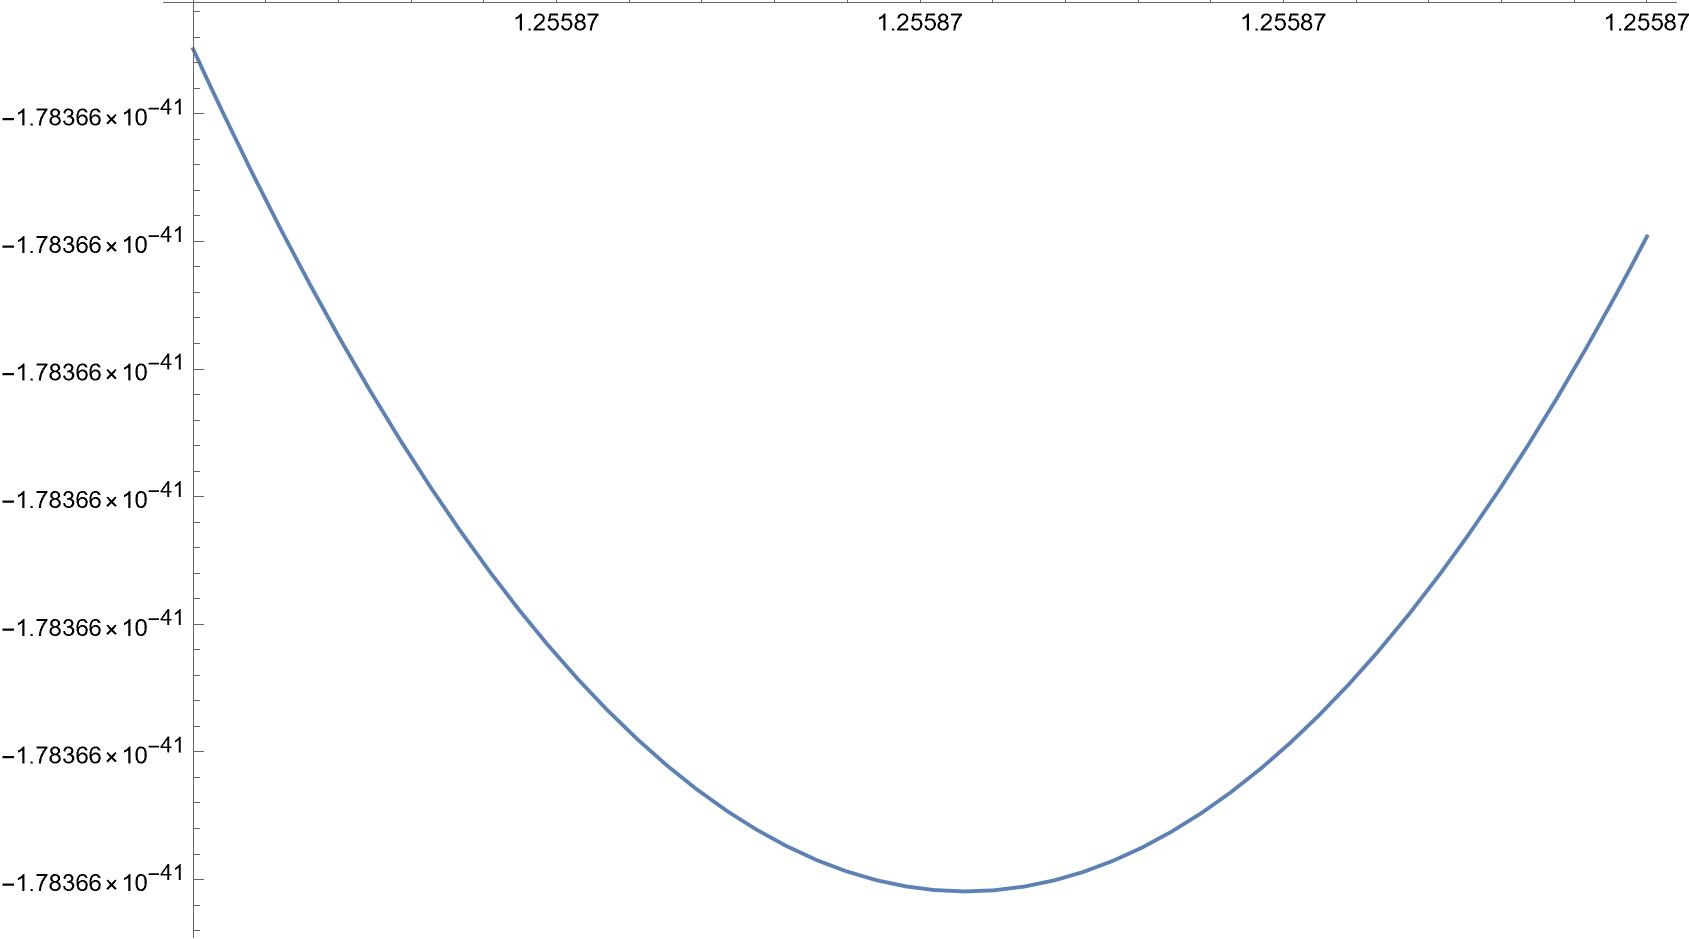
\includegraphics[keepaspectratio,width=0.8\linewidth]{fig/kklt_minimum.jpg}   
   \caption{KKLTモデルのポテンシャル}
   \label{Plot_KKLT}
\end{figure}

次にアップリフティング後のポテンシャル
\begin{equation}
   \left\{
      \begin{alignedat}{1}
         W
         &=
         w_{0}
         -
         Ae^{-aT}
         +
         BX
         \\
         K
         &=
         -
         3\ln(T+\bar{T})
         +
         |X^2|
      \end{alignedat}
   \right.
   \tag*{(\ref{potential_Polonyi-KKLT})}
\end{equation}
を見る.このポテンシャルを
\begin{equation}
   w_{0}
   =
   10^{-20}
   ,\ 
   A=2
   ,\ 
   a=4\pi^2
   ,\ 
   B=10^{-30}
   ,\ 
   X=0
   ,\ 
   \Im T
   =
   0
   \nonumber
\end{equation}
というパラメターでとり,それを$1.25\leq\Re T\leq 1.30$でプロットしたものが図\ref{Plot_Polonyi-KKLT}である.

\begin{figure}[ht]
   \centering
   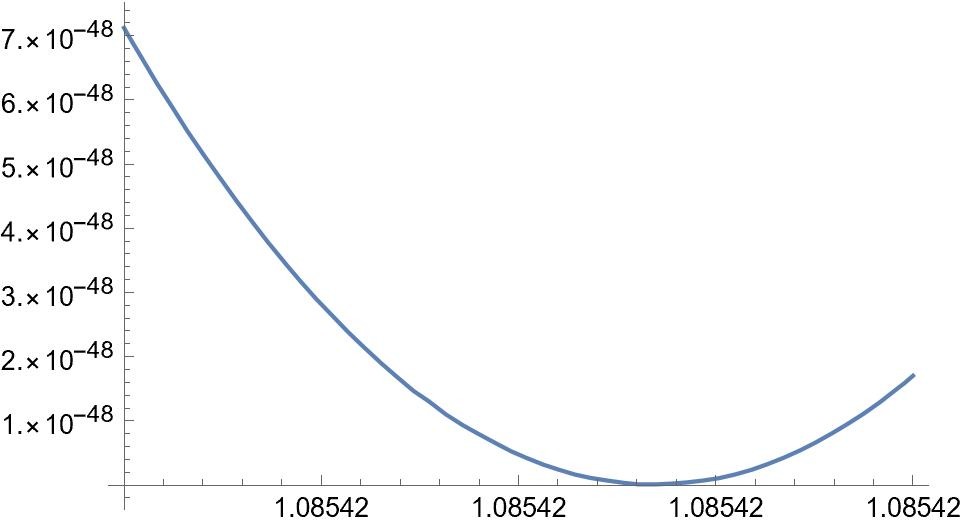
\includegraphics[keepaspectratio,width=0.8\linewidth]{fig/polonyi_kklt_minimum.jpg}   
   \caption{Polonyi-KKLTモデルのポテンシャル($1.25\leq\Re T\leq 1.30$)}
   \label{Plot_Polonyi-KKLT}
\end{figure}

両図を比較すれば分かる通り,最小値が確かにアップリフティングされている.


\subsection*{今回用いる\texorpdfstring{$F$}{F}-termポテンシャル}

今回の研究に用いるポテンシャル
\begin{equation}
   \left\{
      \begin{alignedat}{1}
         W
         &=
         w_{0}
         -
         Ae^{-aT}
         -
         Be^{-bT}X
         \\
         K
         &=
         -
         3\ln(T+\bar{T})
         +
         |X^2|
      \end{alignedat}
   \right.
   \tag*{(\ref{potential_now})}
   \label{potential_now_append}
\end{equation}
を見る.このポテンシャルに対して,
\begin{equation}
   w_{0}
   =
   10^{-30}
   ,\ 
   A=3
   ,\ 
   a=4\pi^2
   ,\ 
   B=0.1
   ,\ 
   b=4\pi^2+30
   ,\ 
   X=0
   ,\ 
   \Im T
   =
   0
   \nonumber
\end{equation}
というパラメターでとり,それを$1.84\leq\Re T\leq 1.96$でプロットしたものが図\ref{Plot_potential_now}である.

\begin{figure}[ht]
   \centering
   \includegraphics[keepaspectratio,width=0.8\linewidth]{fig/polonyi_kklt_mixing_minimum.jpg}   
   \caption{ポテンシャル\ref{potential_now_append}($1.84\leq\Re T\leq 1.96$)}
   \label{Plot_potential_now}
\end{figure}

また,このポテンシャルとパラメターに対して,条件
\begin{equation}
   D_{T}W
   =
   0
   ,\ 
   V^{(F)}_{X}
   =
   0
   \tag*{(\ref{ref_Polonyi-KKLT})}
\end{equation}
を満たす参照点を数値計算で求めたところ,
\begin{equation}
   (t,x)
   \sim
   (1.87688+1.19366i,1.18861 -6.87605i)
   \nonumber
\end{equation}
がその条件を満たす点の1つであった.この点でポテンシャル$V^{(F)}$を展開し,本編の手順によって,変分$\delta T,\delta X$を求めれば
\begin{equation}
   \frac{\delta T}{t}
   \sim
   0.00395
   \ll
   1
   ,\ 
   \frac{\delta X}{x}
   \sim
   0.01275
   \ll
   1
   \nonumber
\end{equation}
となり,近似のコンシステンシーが分かった.この近似が妥当であることは,図\ref{Plot_potential_now}との比較からも分かる.


\clearpage
\bibliography{hoge}
\bibliographystyle{ytphys}

\nocite{柴崎_背景_2021}
\nocite{中野_磁化_2023}

\end{document}
